\documentclass{article}
%IMPORTANT: ONLY INCLUDE AS %IMPORTANT: ONLY INCLUDE AS %IMPORTANT: ONLY INCLUDE AS \input{idp-latex/idp-latex}
\usepackage{import}

\subimport{idp-latex/}{includes-no-theorems}
\subimport{idp-latex/}{theorems}

\usepackage{import}

\subimport{idp-latex/}{includes-no-theorems}
\subimport{idp-latex/}{theorems}

\usepackage{import}

\subimport{idp-latex/}{includes-no-theorems}
\subimport{idp-latex/}{theorems}

\usepackage[breaklinks]{hyperref}
\usepackage{tikz}
\usetikzlibrary{decorations.pathmorphing}

\renewcommand{\sectionautorefname}{Section}

\lstset{basicstyle=\ttfamily,flexiblecolumns=false,captionpos=b}

\begin{document}
\title{\idp: an Unauthorized Tutorial}
\author{Sven Verdoolaege}
\maketitle

\section{Introduction}

\section{Installation}

\idp can be obtained in both source and binary form.
A fairly recent \mbox{C++ 11} compiler is required to compile \idp from source.
For more information on installing \idp, we refer to the reference manual.

\section{Preliminaries}

Recall that a set can be described using either an extensional
or an intensional definition.  In an extensional definition,
the elements of the set are explicitly enumerated.
In an intensional definition, the elements are described
using some properties that they satisfy.
An $n$-tuple, with $n \ge 0$, is an ordered sequence of $n$ elements.
A pair is a 2-tuple.
An $n$-ary relation is a set of $n$-tuples.
A relation is an $n$-ary relation for some $n$.
A predicate is the characteristic function of a relation,
i.e., it is a function that evaluates to true on tuples that belong
to the relation and to false on tuples that do not belong
to the relation.
A proposition is a predicate on a $0$-tuple, i.e.,
it is the characteristic function of a $0$-ary relation.

\section{Knowledge Bases}

A knowledge base deals with several predicates and relations between
these predicates.
The predicates are therefore given names and collected in what
is known as a \emph{structure}.
In particular, a structure is a function from symbols (the names
of the predicates) to $n$-ary relations.
The domain of a structure $S$, i.e., the set of predicate names,
is called the \emph{vocabulary} of the structure and is denoted
$\voc{S}$.  A structure can be considered as an assignment
of the relations to their names and this is also how we will
represent structures in our explanation.
For example, a structure that assigns the empty set to $\mathtt{A}$
and the set containing the $0$-ary tuple to $\mathtt{B}$ is denoted
$$
S =
\{\,
\mathtt{A} \to \{\,\},
\mathtt{B} \to \{\, () \,\}
\,\}
.
$$
The vocabulary of this structure is
$\voc{S} = \{\, \mathtt{A}, \mathtt{B} \,\}$.
The value assigned to name $f$ in $S$ is denoted $S.f$.
For example, $S.\mathtt{A} = \{\,\}$.

Finally, a \emph{knowledge base} $K$ is a set of structures, each
with the same vocabulary.  This shared vocabulary is also called
the vocabulary of the knowledge base $\voc{K}$.
For example, the knowledge base
$$
K = \{\,
\{\, \mathtt{A} \to \{\, \} \,\},
\{\, \mathtt{A} \to \{\, () \,\} \,\}
\,\}
$$
with vocabulary $\{\, \mathtt{A} \,\}$ contains two structures,
one assigning the empty set to $\mathtt{A}$ and
one assigning the set containing the $0$-ary tuple to $\mathtt{A}$.
Note that a knowledge base system such as \idp can be used
to manipulate several knowledge bases and that each of these
knowledge bases may have a different vocabulary.

\idp allows the user to describe the relations inside a structure
either intensionally or extensionally.
Moreover, the knowledge base itself, i.e., the set of structures,
can also be described intensionally or extensionally.
Typically, only some of the
predicates are described extensionally, while everything else
is described intensionally.
In fact, one of the most important operations that can be performed
on such a knowledge base, is to explicitly enumerate some or all of the
structures in the knowledge base.

A knowledge base is often used to describe possible states of the world.
In particular, the predicates inside the structures typically reflect
some properties of the world.  The intensional description of
the knowledge base then describes the constraints that need to
be satisfied by these properties.  In this context, the structures that satisfy
these constraints are the possible states of the world.
Each structure is then also known as a ``possible world''.

\section{Vocabularies}

In \idp, a knowledge base is expressed using three components,
a \texttt{vocabulary}, a \texttt{structure} and a \texttt{theory}.
We first describe \texttt{vocabulary}.
The main purpose of a \texttt{vocabulary} component is to list
the elements of the vocabulary of the knowledge base and to specify
what kind of relation is associated to each predicate name.
The \texttt{structure} and \texttt{theory} components impose
further constraints on the knowledge base.
\texttt{theory}s are first described in \autoref{s:propositional},
while \texttt{structure}s are first described in \autoref{s:enumerations}.

In the simplest case, all predicates are propositions, as in the following
example.
\lstinputlisting[caption={\texttt{voc.idp}},label=l:voc]{tutorial/voc.idp}
Note that we also specified an empty \texttt{structure} and
an empty \texttt{theory}
in the example as most operations in \idp are performed on a pair
of \texttt{theory} and \texttt{structure}.
Since these components are empty, they do not impose any constraints.
Note in particular that a \texttt{structure} component does not
necessarily describe a single structure, but may instead describe
a set of structures.
Each of the components has a name, in this case
\texttt{V}, \texttt{S} and \texttt{T}.
The set of predicates listed in the \texttt{vocabulary} defines
the set of predicates that appears in each structure of the knowledge base.
That is, if $K$ is the knowledge base and $V$ is the set of predicates
listed in the \texttt{vocabulary}, then we have
$$
\voc{K} = V
.
$$
In this example, a $0$-ary relation is
associated with the \texttt{A} identifier, i.e.,
$$
\forall S \in K : S.\mathtt{A} \subseteq \{\, () \,\}
.
$$

The knowledge base contains all structures that satisfy
the above requirements.  In this example, each structure consists
of a single predicate, with two possible values for the relation,
$\{\, \}$ and $\{\, () \,\}$.
This means that the knowledge base contains two structures, i.e.,
$$
K = \{\,
\{\, \mathtt{A} \to \{\, \} \,\},
\{\, \mathtt{A} \to \{\, () \,\} \,\}
\,\}
.
$$

\section{Invoking \idp}

Let us see if we can reproduce this result using \idp.
\idp can be invoked as \texttt{idp}.
We need to tell it where to find the description of the knowledge
base(s) (e.g., \texttt{voc.idp}) and we need to tell \idp what to do with
the knowledge base(s).  The instructions can be included in the input,
they can be specified on the command line or they can be given interactively.
Interactive mode is mostly useful when the description of the knowledge
base is fixed and you want to experiment with different operations
on the knowledge base with different settings (different values of
the options).  However, it is not very convenient when you are still
experimenting with the knowledge base description itself as
\idp is currently unable to forget about components it has seen before.
For example, if you have defined a \texttt{vocabulary} \texttt{V},
then it is impossible to replace it by a new \texttt{vocabulary} with
the same name.
In this tutorial,
we will therefore pass the instructions on the command line,
running a new instance of \idp for each experiment.
The instructions are specified in the Lua language.%
\footnote{\url{http://lua-users.org/wiki/TutorialDirectory}}

The procedure for explicitly listing all the structures
in a knowledge base is called \lstinline{modelexpand}.
This procedure takes a \texttt{theory} and a \texttt{structure}
that are defined over the same \texttt{vocabulary} (with the same name)
as arguments
and produces a list of all the structures that satisfy the
constraints specified in the \texttt{vocabulary}, the \texttt{structure}
and the \texttt{theory}.
By default, \lstinline{modelexpand} will truncate the list
of structures to a list of at most one element because it can
be quite expensive to compute all structures and because in many
cases the user is only interested in a single structure.
The default can be changed by setting the
\lstinline{stdoptions.nbmodels} option.  The value \lstinline{0}
means that all structures should be computed and returned.

The following transcript shows how we can print the number
of structures found, where \texttt{voc.idp} is the name of a file
containing the contents of \autoref{l:voc}.
\begin{lstlisting}{}
$ idp -e 'stdoptions.nbmodels=0;
    L=modelexpand(T,S);print(#L);' voc.idp 
2
\end{lstlisting}
When \idp is invoked in this way, it
first reads the contents of the file \texttt{voc.idp}
and constructs an internal representation of the components in the file.
For each component with name $n$, \idp assigns a reference to the
corresponding object to the Lua variable with the same name, i.e., $n$.
It is, however, important to keep in mind that the Lua variable
and the object are not the same and that one just refers to the other.
In particular, the user may assign a different value to the Lua
variable and this will not affect the object.  If this was the last
reference to the object, then it will become unreachable, but it will
not be removed and it can then also not be replaced by another object
with the same name.
After parsing the input file, \idp continues with the execution of
the commands passed through the \lstinline{-e} option.
The first command \lstinline{stdoptions.nbmodels=0} sets
the \lstinline{stdoptions.nbmodels} to \lstinline{0}.
The second command \lstinline{L=modelexpand(T,S)} applies
\lstinline{modelexpand} to the theory and structure referenced
by the Lua variables \lstinline{T} and \lstinline{S} (at this stage,
these variables refer to the \lstinline{theory} and \lstinline{structure}
in \lstinline{voc.idp} of the same names) and stores the result
(an array of structures) in the Lua variable \lstinline{L}.
The final command \lstinline{print(#L)} prints the number of elements
in the array (or ``table'' in Lua-speak) \lstinline{L}.
Notice that \idp has indeed found two structures in the knowledge base.

The actual structures can be printed as follows
\begin{lstlisting}{}
$ idp -e 'stdoptions.nbmodels=0;
    L=modelexpand(T,S);
    for i=1,#L do print (L[i]) end' voc.idp 
structure  : V {
  A = true
}

structure  : V {
  A = false
}

\end{lstlisting}
As can be seen from the instructions, the array
returned by \lstinline{modelexpand}
starts at index 1 (which is the default in Lua).
Each structure is represented as an anonymous \texttt{structure} over the same
\texttt{vocabulary} as the input \texttt{structure} and \texttt{theory}.
In this output, each of the \texttt{structure}s \emph{does} represent
a single structure.
Note that structures are not generated in any fixed order,
so you may receive them in a different order from the one in the output
above.
We will describe the various elements of a \texttt{structure} in more
detail later.  Here, the predicate \texttt{A} is simply enumerated.
Note that \texttt{true} is an alternative notation
for \lstinline!{()}!, while \texttt{false} is an alternative notation
for \lstinline!{}!.

\section{Propositional Constraints}\label{s:propositional}

Up until now, we have only seen how to specify that a predicate
should exist in all structures, but we have not explained how
to affect the values of the predicates.
One way of doing so is by imposing constraints on them.
These constraints are specified in first-order logic and appear
in a \texttt{theory}.
The textual representations of the standard connectives
in \idp are shown in \autoref{t:connectives}.
Notice in particular that \texttt{<=} means ``is implied by''
and does not mean ``is less than or equal to''.
Since we have only explained how to declare propositions,
the connectives $\exists$ and $\forall$ will only become useful
in \autoref{s:first-order}.
Each constraint is terminated by a ``\texttt{.}''.

\begin{table}
\begin{center}
\begin{tabular}{c|c|l}
Logic & \idp & Declarative reading \\
\hline
$\land$    & \code{ \&}  & and \\
$\lor$    & \code{ |}  & or  \\
$\lnot$    & \code{$\sim$}  & not \\
$\limplies$    & \code{ =>}  & implies \\
$\limpliedby$    & \code{ <=}  & is implied by \\
$\lequiv$    & \code{ <=>}  & is equivalent to \\
$\forall$  & \code{ !}  & for each \\
$\exists$  & \code{ ?}  & there exists \\
$=$      & \code{ =}  & equals \\
$\neq$    & \code{$\sim$=}  & does not equal \\ 
\end{tabular}
\end{center}
\caption{Connectives in \idp}
\label{t:connectives}
\end{table}

As a simple example, consider the following input.
\lstinputlisting[caption={\texttt{con1.idp}}]{tutorial/con1.idp}
Without the constraint, there are four structures in the knowledge base.
The constraint eliminates one of them (the one where
\texttt{A} is \texttt{true} and \texttt{B} is \texttt{false}),
leaving three structures as shown in the following transcript.
\begin{lstlisting}{}
$ idp -e 'stdoptions.nbmodels=0;
    L=modelexpand(T,S);
    for i=1,#L do print (L[i]) end' con1.idp 
structure  : V {
  A = false
  B = false
}

structure  : V {
  A = false
  B = true
}

structure  : V {
  A = true
  B = true
}

\end{lstlisting}

\section{Built-in Types}

Predicates in \idp need to be typed.  For the propositions we have
seen so far, this was not needed because they have zero arguments,
but as soon as we want to deal with predicates with one or more arguments,
we need to specify the types of these arguments.
Types can be built-in or user-defined.
In the current version of \idp, all types are subsets of
the built-in types \texttt{float} or \texttt{string}.
The remaining built-in types are \texttt{nat}, \texttt{int} and
\texttt{char}.  \texttt{int} and \texttt{nat} are subtypes of
\texttt{float} representing the integers and the non-negative
integers, respectively.  \texttt{char} is a subtype of \texttt{string}
containing the single character strings.
Of these types, only \texttt{char} is finite, while the remaining
built-in types are infinite.%
\footnote{Technically, \idp only supports integers of a fixed width,
so only a finite number of integers are representable.  Similarly,
the maximal length of the strings is bounded.}
In particular, the \texttt{char} type contains 256 elements.
Since current versions of \idp do not handle infinite types very well,
we will only use the \texttt{char} type, until we explain how
to specify user-defined types in \autoref{s:user-defined}.

The types of the predicates are specified by listing the types
of the arguments to the predicates.  For example,
\begin{lstlisting}{}
vocabulary V {
  A(char)
  B(char,char)
}
\end{lstlisting}
imposes the constraints
$$
\forall S \in K : S.\mathtt{A} \subseteq {\cal C}
$$
and
$$
\forall S \in K : S.\mathtt{B} \subseteq {\cal C} \times {\cal C}
,
$$
where $\cal C$ is the set of characters.
In the special case of propositions, i.e., predicates with zero arguments,
the ``\texttt{()}'' are optional.  That is, \texttt{A} in \autoref{l:voc}
could also have been written as \texttt{A()}.

It should be noted that the built-in types are imported into
every \texttt{vocabulary} from a predefined \texttt{std} \texttt{vocabulary},
which means that their canonical names are \texttt{std::char}, \ldots.
Furthermore, it is possible to overload predicates with the same names,
but with different arguments.  The fully qualified names of the predicates
contain the names of the argument types.  For example, the
fully qualified name of the \texttt{A} predicate above is
\texttt{A[std::char]}.
The fully qualified name only needs to be used in case of ambiguity.

\section{First-Order Constraints}
\label{s:first-order}

Now that we have seen how to declare predicates with one or more
arguments, we can consider some slightly more interesting constraints.
As a first example, consider the following input.
\lstinputlisting[caption={\texttt{con2.idp}},label=l:con2]{tutorial/con2.idp}
The constraint imposes that \texttt{A} holds for the element \lstinline!"a"!.
Nothing is said about any of the other characters.
The predicate \texttt{A} may or may not hold for those elements.
This means that there are a total of $2^{255}$ structures.
It is therefore not a good idea to try and explicitly compute
all structures in the knowledge base.
The transcript below shows how to compute one of
them.  You may very well obtain a different structure.
\begin{lstlisting}{}
$ idp -e 'print (modelexpand(T,S)[1])' con2.idp 
structure  : V {
  A[std::char] = { a }
}

\end{lstlisting}
Recall that by default \texttt{modelexpand} computes a single structure
of the knowledge base.

We can eliminate some of the structures by adding additional constraints.
We may, for example, impose that \texttt{A} holds for only a single
element of \texttt{char}.  There are several ways of expressing
this constraint.  One is to say that if \texttt{A} holds for two elements
then they have to be the same, as in the following input.
\lstinputlisting[caption={\texttt{con3.idp}},label=l:con3]{tutorial/con3.idp}
All variables that appear in a constraint need to be quantified and typed.
Explicit typing is performed by appending the name of the type in square
brackets to the variable.  Typing may also be performed implicitly by
having \idp guess the types of the variables from the types of the predicates
where they are used.  This may sometimes lead to surprising results, however,
so it is better to always type the variables explicitly.

\begin{table}
\begin{center}
\begin{tabular}{c|c|l}
\idp & Declarative reading \\
\hline
\code{?n}  & there exist exactly $n$ different elements such that \\
\code{?<n} & there exist less than $n$ \\
\code{?=<n} & there exist at most $n$\\
\code{?=n} & there exist exactly $n$ (this is the same as \code{?n})\\
\code{?>n} & there exist more than $n$
\end{tabular}
\end{center}
\caption{Counting quantifiers in \idp}
\label{t:counting}
\end{table}

Another way of expressing the same constraint is to use counting quantifiers.
In particular, we can state that there is exactly one element of
\texttt{char} for which \texttt{A} holds, as in the following input.
\lstinputlisting[caption={\texttt{con4.idp}},label=l:con4]{tutorial/con4.idp}
The counting quantifiers supported by \idp are shown in
\autoref{t:counting}.

\section{Definitions}\label{s:definitions}

First-order constraints form an indirect way of specifying
for which tuples a predicate holds.
It is also possible to stipulate exactly which tuples
belong to a predicate through a definition.
A definition defines one or more predicates and has the following
form
\begin{lstlisting}[escapechar=@]{}
  {
    !@\it{variables}@ @\it{predicate}@ <- @\it{formula}@.
    @\it{predicate}@ <- @\it{formula}@.
    !@\it{variables}@ @\it{predicate}@.
    @\it{predicate}@.
    @\ldots@
  }
\end{lstlisting}
If \textit{formula} is \texttt{true}, then it may be omitted, along with
the \texttt{<-}.  If there are no variables in the rule, then the
quantifier should be dropped.

In the simplest case, there are no variables and the formula is
(implicitly) \texttt{true}.  In this case, the definition simply
enumerates the tuples for which the predicate holds.
For example, the following input defines the \texttt{A} predicate
as holding for \texttt{"a"} (and nothing else).
It is therefore equivalent to the inputs in \autoref{l:con3}
and \autoref{l:con4}.
\lstinputlisting[caption={\texttt{def1.idp}}]{tutorial/def1.idp}
Notice the difference with the input in \autoref{l:con2}.
Recall that the input in \autoref{l:con2} only imposes that \texttt{A} holds
for the element \lstinline!"a"!, but does not say anything about any
other characters, while the input above specifies exactly for which
characters \texttt{A} holds.

\begin{figure}
\centering%
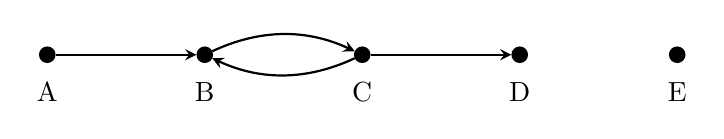
\begin{tikzpicture}[x=1.0cm,y=.6cm,>=stealth,shorten >=3pt,shorten <=3pt]
\foreach \i in {1,...,5}{ \fill (2*\i,0) circle(3pt); }
\draw[->,thick](2,0) to (4,0);
\draw[->,thick](4,0) to [out=25,in=155] (6,0);
\draw[->,thick](6,0) to [out=-155,in=-25] (4,0);
\draw[->,thick](6,0) to (8,0);
\draw (2,-0.8) node {A};
\draw (4,-0.8) node {B};
\draw (6,-0.8) node {C};
\draw (8,-0.8) node {D};
\draw (10,-0.8) node {E};
\end{tikzpicture}
\caption{A simple graph}
\label{f:graph}
\end{figure}

As a slightly more interesting example, consider the (directed)
graph in \autoref{f:graph}.  We can define a predicate \texttt{node}
for all nodes in the graph and a predicate \texttt{edge} for all
pairs of nodes connected by an edge as follows.
\lstinputlisting[caption={\texttt{graph.idp}},label=l:graph]{tutorial/graph.idp}
Note that we have used two definitions in this example, one for
each predicate.  It would have been possible to define these two
predicates in a single definition, but since they do not depend
on each other there is no need to do so.
Note that just like the first-order constraints, each definition
imposes a constraint on the structures in the knowledge base.
In this case, the conjunction of the constraints imposed by
the two definition is the same as the constraint imposed by
a definition that would define both predicates.

A definition can also be used to define a predicate in terms
of one or more predicates, possibly including the predicate that
is being defined itself.
For example, we may want to say that two nodes are adjacent
to each other if there is an edge from one of the two nodes
to the other.  This concept can be defined using the following
definition.
\begin{lstlisting}{}
  {
    !x[char], y[char] : adjacent(x,y) <-
				edge(x,y) | edge(y,x).
  }
\end{lstlisting}
The meaning of such a definition is that set of tuples $(x,y)$
for which \texttt{adjacent(x,y)} holds is defined to be those
for which \texttt{edge(x,y) | edge(y,x)} holds.
If there is more than one rule defining the same predicate,
then the predicate is defined to hold for those tuples where
the disjunction of the formulas holds.
That is, the definition above is equivalent to
\begin{lstlisting}{}
  {
    !x[char], y[char] : adjacent(x,y) <- edge(x,y).
    !x[char], y[char] : adjacent(x,y) <- edge(y,x).
  }
\end{lstlisting}
Similarly, the definition of \texttt{node} in \autoref{l:graph}
is equivalent to the following definition.
\begin{lstlisting}{}
  {
    !x[char] : node(x) <- x = "A" | x = "B" | x = "C" |
			  x = "D" | x = "E".
  }
\end{lstlisting}

Adding the \texttt{adjacent} definition to the input in \autoref{l:graph} and
adding \texttt{adjacent}
to the vocabulary results in the input shown in \autoref{l:adjacent}.
The input defines a knowledge base containing a single structure,
which is printed by \idp
as follows (reformatted to fit the page width).
\begin{lstlisting}{}
structure  : V {
  adjacent[std::char,std::char] =
		    { A,B; B,A; B,C; C,B; C,D; D,C }
  edge[std::char,std::char] = { A,B; B,C; C,B; C,D }
  node[std::char] = { A; B; C; D; E }
}

\end{lstlisting}
As can be seen, the tuples for which the predicates hold are separated
by a \lstinline{;}.  In particular, the \texttt{adjacent} predicate
holds for the tuples
(\texttt{"A","B"}),
(\texttt{"B","A"}),
(\texttt{"B","C"}),
(\texttt{"C","B"}),
(\texttt{"C","D"}) and
(\texttt{"D","C"}),
as expected.

\lstinputlisting[float,caption={\texttt{adjacent.idp}},label=l:adjacent]
	{tutorial/adjacent.idp}

The real power of definitions only comes into play when
a predicate is defined (possibly indirectly) in terms of itself.
The prototypical example of such a definition is the transitive closure.
In the case of graphs, the transitive closure can be applied to edges,
resulting in the concept of reachability.
In particular, we say that there is a path from $x$ to $y$ if there
is an edge from $x$ to $y$ or if there is some node $z$ such that there
is a path from $x$ to $z$ and a path from $z$ to $y$.
That is, \texttt{path} can be defined as follows.
\begin{lstlisting}{}
  {
    !x[char], y[char] : path(x,y) <- edge(x,y).
    !x[char], y[char] : path(x,y) <-
		    ?z[char] : path(x,z) & path(z,y).
  }
\end{lstlisting}
An equivalent definition, where one of the \texttt{path}s
is replace by an \texttt{edge} and which can be handled more efficiently,
is as follows.
\begin{lstlisting}{}
  {
    !x[char], y[char] : path(x,y) <- edge(x,y).
    !x[char], y[char] : path(x,y) <-
		    ?z[char] : edge(x,z) & path(z,y).
  }
\end{lstlisting}
Adding this definition to the input in \autoref{l:graph} and
adding \texttt{path}
to the vocabulary results in the input shown in \autoref{l:path}.
The input defines a knowledge base containing a single structure,
which is printed by \idp
as follows (reformatted to fit the page width).
\begin{lstlisting}{}
structure  : V {
  edge[std::char,std::char] = { A,B; B,C; C,B; C,D }
  node[std::char] = { A; B; C; D; E }
  path[std::char,std::char] = { A,B; A,C; A,D; B,B;
			    B,C; B,D; C,B; C,C; C,D }
}

\end{lstlisting}

\lstinputlisting[float,caption={\texttt{path.idp}},label=l:path]
	{tutorial/path.idp}

It is important to understand that a definition is different from
an equivalence.  An equivalence only expresses that either both
sides are \texttt{false} or both sides are \texttt{true}.
In a definition, a true right hand side \emph{causes} the left hand side
to be true.  For each true left hand side, there must be an explanation
of why that left hand side came to be true.
For example, if the \texttt{path} definition is replaced by the following
equivalence,
\begin{lstlisting}{}
  !x[char], y[char] : path(x,y) <=>
        edge(x,y) | ?z[char] : edge(x,z) & path(z,y).
\end{lstlisting}
then the resulting input allows for a structure of the following
form.
\begin{lstlisting}{}
structure  : V {
  edge[std::char,std::char] = { A,B; B,C; C,B; C,D }
  node[std::char] = { A; B; C; D; E }
  path[std::char,std::char] = { A,B; A,C; A,D; A,E; B,B;
		    B,C; B,D; B,E; C,B; C,C; C,D; C,E }
}
\end{lstlisting}
Notice that in this structure, \texttt{path} also holds
for the tuples \texttt{(A,E)}, \texttt{(B,E)} and \texttt{(C,E)}.
This result is consistent with the equivalence, but not with the definition
because it can only be explained through circular reasoning.
That is, \texttt{path(B,E)} could be explained based on
\texttt{edge(B,C)} and \texttt{path(C,E)}, but the only way to explain
\texttt{path(C,E)} would be to make use of \texttt{path(B,E)}.
A definition does not allow such circular reasoning.

Note that causality only plays a role \emph{within} a definition.
That is, the definition
\begin{lstlisting}{}
  {
    p <- q.
    q <- p.
  }
\end{lstlisting}
is \emph{not} equivalent to the \emph{pair} of definitions
\begin{lstlisting}{}
  {
    p <- q.
  }
  {
    q <- p.
  }
\end{lstlisting}
The single definition only allows for a single structure,
one where both \texttt{p} and \texttt{q} are \texttt{false}, because
there is no way to explain either \texttt{p} or \texttt{q} being
\texttt{true} except through circular reasoning.
The pair of definitions also allows for the structure where
both \texttt{p} and \texttt{q} are \texttt{true}.
In the first definition \texttt{p} can be explained because of \texttt{q},
while, independently, in the second definition,
\texttt{q} can be explained because of \texttt{p}.
In this case then the conjunction of the constraints imposed
by the two separate definitions is not equivalent to the constraint
imposed by the single combined definition.

Finally, it should be noted that the right hand side of a definition
includes an implicit condition that all the arguments that appear
on the left hand side are of the appropriate type.
Consider, for example, the following input.
\lstinputlisting[caption={\texttt{def2.idp}}]{tutorial/def2.idp}
The rule ``\lstinline{P("string").}'' in the definition in this input
is interpreted as the rule ``\lstinline{P("string") <- char("string").}''.
Since \lstinline{"string"} does not belong to the type \lstinline{char},
it is not made to satisfy \texttt{P}.
The input therefore defines a single structure in which \texttt{P}
is empty.

\section{Enumerations}\label{s:enumerations}

In \autoref{s:definitions}, we have seen how definitions can
be used to enumerate the tuples for which a predicate holds.
Such enumerating definitions can be expressed more succinctly
by providing an extensional description of the associated relation
in the \texttt{structure}.
For example, the following input is equivalent to that in
\autoref{l:graph}.
\lstinputlisting[caption={\texttt{graph2.idp}},label=l:graph2]
	{tutorial/graph2.idp}

The syntax should look familiar, as it is the same as that
used to represent structures in the output of \lstinline{modelexpand}.
In particular, the elements in the tuples are separated by ``\texttt{,}''
while the tuples themselves are separated by ``\texttt{;}''.
The meaning of, say, the enumeration of \texttt{node} is simply,
$$
\forall S \in K : S.\mathtt{node} =
\{\, \texttt{"A"},\texttt{"B"},\texttt{"C"},\texttt{"D"},\texttt{"E"} \,\}
.
$$

\section{User-defined Types}\label{s:user-defined}

A user-defined type is essentially a unary predicate that is preceded
in the \texttt{vocabulary} by the keyword \texttt{type}.
The elements of the type need to be enumerated, either explicitly
or implicitly, in the \texttt{structure}.
Explicit enumerations are performed as in \autoref{s:enumerations}.
If the \texttt{structure} does not contain an explicit enumeration
of a type, then the type is defined as containing those elements
that are used inside the \texttt{structure} where an element of the
type is expected.
For example, the following input is equivalent to that in
\autoref{l:graph} and \autoref{l:graph2}.
\lstinputlisting[caption={\texttt{graph3.idp}},label=l:graph3]
	{tutorial/graph3.idp}
It would be possible to leave out the enumeration of \texttt{node},
but then it would not contain \texttt{"E"} as the node \texttt{"E"}
does not appear in any of the edges.

When declaring a type, it is possible to indicate that the new type
is a subset (\texttt{isa}) or a superset (\texttt{contains}) of one
or more other previously declared types.
That is, a declaration of the form
\begin{lstlisting}{}
  type t1 isa t2
\end{lstlisting}
declares the type \texttt{t1} and imposes the constraint
$$
\forall S \in K : S.\mathtt{t1} \subseteq S.\mathtt{t2}
.
$$

Declaring a type to be a subset (directly or indirectly) of a built-in
type, allows elements of that built-in type to be used in places
where elements of the user-defined type are expected in the
\texttt{theory}.

\section{Bounds}

\begin{figure}
\centering%
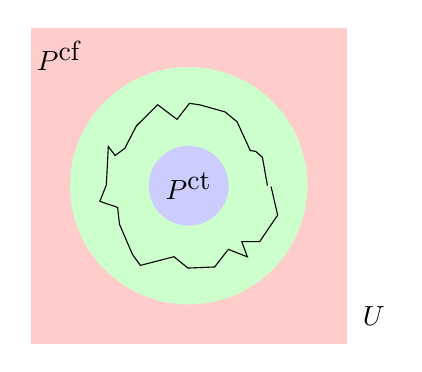
\begin{tikzpicture}
\draw[fill,red!20] (-2,-2) rectangle (2,2);
\draw[fill,green!20] (0,0) circle (1.5cm);
\draw[fill,blue!20] (0,0) circle (0.5cm);
\draw[decorate, decoration={random steps,segment length=6pt,amplitude=5pt}]
    (0,0) circle (1cm);
\draw (0,0) node {$P^{\textrm{ct}}$};
\draw (-1.65,1.65) node {$P^{\textrm{cf}}$};
\draw (2.35,-1.65) node {$U$};
\end{tikzpicture}
\caption{Bounds on a predicate $P$.  $P$ is represented by the squiggly line.
The set $P^{\textrm{ct}} \subseteq P$ is represented by the innermost (blue)
circle.  The set $P^{\textrm{cf}}$ with
$P \subseteq U \setminus P^{\textrm{cf}}$ is represented by the (red) region
outside the outer circle.  The (green) band between the two circles
represents $P^{\textrm{u}}$.} 
\label{f:bounds}
\end{figure}

A \texttt{structure} can not only be used to explicitly enumerate
predicates, it can also be used to specify bounds on a predicate.
Every predicate $P$ is typed and therefore is a subset of some
universe $U$ that is the Cartesian product of the types of its
arguments.  It is possible to specify which elements ($P^{\textrm{ct}}$)
of $U$ certainly
satisfy the predicate, which elements ($P^{\textrm{cf}}$) certainly
do not satisfy
the predicate and which elements ($P^{\textrm{u}}$)
may or may not satisfy the predicate.
The relationship between these relations is illustrated in
\autoref{f:bounds}.  Since the three relations partition $U$ and
$U$ is known, only two of the relations need to be specified.
In particular, they can be specified by appending
\texttt{<ct>},
\texttt{<cf>} or
\texttt{<u>} to the predicate name.
If $R_1$ is the relation listed for \texttt{P<ct>} and
$R_2$ is the relation listed for \texttt{P<cf>}
then the constraint imposed by these two enumerations is
$$
\forall S \in K : R_1 \subseteq S.\mathtt{P}
  \wedge S.\mathtt{P} \cap R_2 = \emptyset
.
$$

While in many ways, a type behaves similarly to a unary predicate,
it is not allowed to specify bounds on a type.

\section{Functions}

A function can be declared in a \texttt{vocabulary} as follows.
\begin{lstlisting}[escapechar=@]{}
vocabulary V {
  @$f$@(@$t_1$@, @$t_2$@, @\ldots@, @$t_n$@) : @$t_0$@
}
\end{lstlisting}
Such a declaration adds a $(n+1)$-ary predicate to the structures
where the final argument is uniquely determined by the previous arguments,
i.e.,
$$
\forall S \in K : S.f \subseteq
	t_1 \times t_2 \times \ldots \times t_n \times t_0
$$
and
$$
\begin{aligned}
& \forall S \in K :
	\forall (u_1, u_2, \ldots, u_n, u_0),
	(v_1, v_2, \ldots, v_n, v_0) \in S.f: \\
&	u_1 = v_1 \wedge u_2 = v_2 \wedge \ldots \wedge u_n = v_n
	\Rightarrow u_0 = v_0
.
\end{aligned}
$$
For example, we may want to assign a color to the nodes
of the graph example in \autoref{l:graph3}.  The \texttt{node\_color}
function could then be declared as follows.
\begin{lstlisting}{}
vocabulary V {
  type node
  type color
  edge(node, node)
  node_color(node) : color
}
\end{lstlisting}

Functions can be enumerated inside a \texttt{structure} using the following
syntax.
\begin{lstlisting}[escapechar=@]{}
structure S {
  @$f$@ = { @$v_1$@, @$v_2$@, @\ldots@, @$v_n$@ -> @$v_0$@; @\ldots@ }
}
\end{lstlisting}
For example, the \texttt{node\_color} function could be enumerated as follows.
\begin{lstlisting}{}
  node_color = { "A" -> "red"; "B" -> "blue";
	"C" -> "green"; "D" -> "blue"; "E" -> "red" }
\end{lstlisting}
If a function is enumerated, then it needs to enumerated completely.
That is, each element of the domain should be assigned a value.

Inside a \texttt{theory}, a function applied to a tuple is interpreted
as the value assigned to that tuple by the function.
For example, we can extend the example in \autoref{l:graph3} to
a graph coloring problem by adding the following constraint.
\begin{lstlisting}{}
  !x[node] y[node] :
    edge(x,y) => node_color(x) ~= node_color(y).
\end{lstlisting}
The complete input is shown in \autoref{l:coloring}.
One of the structures found by \idp is the following.
\begin{lstlisting}{}
structure  : V {
  V::color[V::color] = { blue; green; red }
  V::node[V::node] = { A; B; C; D; E }
  edge[V::node,V::node] = { A,B; B,C; C,B; C,D }
  node_color[V::node:V::color] = { A->blue; B->red;
			C->green; D->blue; E->blue }
}
\end{lstlisting}

\lstinputlisting[float,caption={\texttt{coloring.idp}},label=l:coloring]
	{tutorial/coloring.idp}

A function with zero arguments is called a ``constant''.
It is important to understand that such ``constants'' are only constant
inside any given structure and that they may have different values
across different structures in the same knowledge base.
The ``enumeration'' of a constant can be expressed using a simplified
syntax, as illustrated by the following example.
\begin{lstlisting}{}
vocabulary V {
  f : char
}
structure S : V {
  f = "A"
}
\end{lstlisting}
Note that if a constant is ``enumerated'' then it will have the
same value (the value assigned in the enumeration) in all structures
of the knowledge base.

If a user-defined type is declared to be a subtype of a built-in type,
then \idp will allow variables or elements of that built-in type to
be used in positions in the \texttt{theory} where the user-defined
type is expected.  A function may then end up getting applied
to elements outside its domain.
Future versions of \idp will detect such situations, but currently
it is up to the user to avoid them.
In particular, an occurrence of a function application
$P(\ldots,F(x),\ldots)$ where $F$ may or may not be defined on $x$
is not allowed and should be replaced by either
$$\exists y\ (F(x) = y \land P(\ldots,y,\ldots))$$
or
$$\forall y\ (F(x) = y \limplies P(\ldots,y,\ldots)).$$
Note that a formula of the form
$$
F(x) = y,
$$
where $y$ is either a variable or an element from a built-in type,
is only true if the function $F$ is defined at $x$.

Note that \idp also allows for partial functions that may only be
defined on a subset of the declared domain.  Such partial functions
are declared using the \texttt{partial} keyword.
For example, we may allow that only some (or even none) of the nodes
have a color assigned to them by declaring \lstinline{node_color} as follows.
\begin{lstlisting}{}
  partial node_color(node) : color
\end{lstlisting}

\section{Aggregates}

While most constraints in a \texttt{theory} are first-order constraints,
it is also possible to place constraints on certain properties of sets
through aggregates.
Arguably the simplest aggregate is the cardinality of a set.
This aggregate can be used to count the number of elements that
satisfy a property.
The cardinality of the set
$$
\{\,
(v_1, v_2, \ldots, v_n) \in t_1 \times t_2 \times \ldots \times t_n \mid
\phi(v_1, v_2, \ldots, v_n)
\,\}
$$
is represented as
\begin{lstlisting}[escapechar=@]{}
card { @$v_1$@[@$t_1$@] @$v_2$@[@$t_2$@] @\ldots@ @$v_n$@[@$t_n$@] : @$\phi(v_1, v_2, \ldots, v_n)$@ }
\end{lstlisting}
For example, in the coloring example of \autoref{l:coloring},
we may want to impose that at least two nodes are colored red.
\begin{lstlisting}{}
  card { x[node] : node_color(x) = red } >= 2.
\end{lstlisting}
Here, \texttt{red} is a constant of type \texttt{color}.
The complete input is shown in \autoref{l:coloring2}.
One of the structures in the knowledge base found by \idp is as follows.
\begin{lstlisting}{}
structure  : V {
  V::color[V::color] = { blue; green; red }
  V::node[V::node] = { A; B; C; D; E }
  edge[V::node,V::node] = { A,B; B,C; C,B; C,D }
  node_color[V::node:V::color] = { A->red; B->green;
			    C->red; D->blue; E->blue }
  red[:V::color] = red
}
\end{lstlisting}

\lstinputlisting[float,caption={\texttt{coloring2.idp}},label=l:coloring2]
	{tutorial/coloring2.idp}

The other aggregates compute a reduction of an operator over
an integer expression associated to each element of a set.
The operator may be one of \texttt{sum},
\texttt{prod} (product), \texttt{min} (minimum) or \texttt{max} (maximum).
The expression
$$
\min_{
\{\,
(v_1, v_2, \ldots, v_n) \in t_1 \times t_2 \times \ldots \times t_n \mid
\phi(v_1, v_2, \ldots, v_n)
\,\}} e(v_1, v_2, \ldots, v_n)
$$
is represented as
\begin{lstlisting}[escapechar=@]{}
min { @$v_1$@[@$t_1$@] @$v_2$@[@$t_2$@] @\ldots@ @$v_n$@[@$t_n$@] : @$\phi(v_1, v_2, \ldots, v_n)$@ : @$e(v_1, v_2, \ldots, v_n)$@ }
\end{lstlisting}
and similarly for the other operators.
For example, the cardinality constraint in the previous example
can be rewritten as follows.
\begin{lstlisting}{}
  sum { x[node] : node_color(x) = red : 1 } >= 2.
\end{lstlisting}

\section{Optimization}

Up until now, we have only used the \texttt{modelexpand} procedure,
but \idp provides several other procedures.
One of these is the \texttt{minimize} procedure which is used not to compute
\emph{all} structures that satisfy the constraints in the input,
but only those that minimize a given integer expression.
The integer expression needs to be specified in a \texttt{term} block
in the input.
For example, we may introduce a \texttt{term} for the number
of blue nodes as follows.
\begin{lstlisting}{}
term n_blue : V {
  card { x[node] : node_color(x) = blue } 
}
\end{lstlisting}
The complete input is shown in \autoref{l:coloring3}.
The following transcript shows how we can print a
structure where this number of blue nodes is minimized.
\begin{lstlisting}{}
$ idp -e 'print (minimize(T,S,n_blue)[1])' \
	coloring3.idp 
structure  : V {
  V::color[V::color] = { blue; green; red }
  V::node[V::node] = { A; B; C; D; E }
  edge[V::node,V::node] = { A,B; B,C; C,B; C,D }
  blue[:V::color] = blue
  node_color[V::node:V::color] = { A->red; B->green;
			C->red; D->green; E->green }
  red[:V::color] = red
}
\end{lstlisting}
The minimal number of blue nodes turns out to be zero in this example.

\lstinputlisting[float,caption={\texttt{coloring3.idp}},label=l:coloring3]
	{tutorial/coloring3.idp}

\end{document}
